\documentclass[a4paper,twoside,spanish,12pt]{report}
\usepackage{pslatex} %utilizar fuentes postscript standard
\usepackage[T1]{fontenc} %codificacion de tipo
\usepackage[spanish]{babel}
\usepackage[latin1]{inputenc} %entrada usando ISO-Latin1
\usepackage{makeidx} %para los indices
\usepackage{amssymb}
\usepackage{amsmath}
\usepackage{euler}
\usepackage{a4wide}
%\oddsidemargin 2.5cm
\usepackage{subfigure}
\usepackage{graphicx}
  \graphicspath{{figures/}}
\usepackage{array}
\providecommand{\tabularnewline}{\\}


\usepackage[boxed,section]{algorithm}
\usepackage{algpseudocode}
\floatname{algorithm}{Algoritmo}
\renewcommand{\listalgorithmname}{Lista de algoritmos}
\usepackage{makeidx}
%\usepackage{hyperref}
%\hypersetup{colorlinks,%
%            pdftex,%
%            linkcolor=black,%
%            citecolor=black,%
%            filecolor=black,%
%            urlcolor=black,%
%						pdfpagemode={None}		}
\frenchspacing
\usepackage[amsmath,framed,thref,hyperref]{ntheorem}

\theoremstyle{break}
\theoremheaderfont{\normalfont\bfseries}
\theorembodyfont{\slshape}
\theoremseparator{:}
\newtheorem{teorema}{Teorema}[section]
\newtheorem{proposicion}{Proposici�n}[section]
\newtheorem{lema}{Lema}[section]
\newtheorem{observacion}{Observaci�n}[section]
\newtheorem{corolario}[teorema]{Corolario}
\theoremseparator{.}
%\theoremprework{\bigskip\hrule}
%\theorempostwork{\hrule\bigskip}
\newtheorem{definicion}{Definici�n}[section]

\theoremstyle{change}
\theorembodyfont{\upshape}
\theoremseparator{}
\newtheorem{ejemplo}{Ejemplo}

\theoremstyle{nonumberplain}
\theoremseparator{}
\theoremprework{\relax}
\theorempostwork{\relax}
\newtheorem{demostracion}{Demostraci�n}

 \newenvironment{lyxcode}
   {\begin{list}{}{
     \setlength{\rightmargin}{\leftmargin}
     \setlength{\listparindent}{0pt}
     \raggedright
     \setlength{\itemsep}{0pt}
     \setlength{\parsep}{0pt}
     \normalfont\ttfamily}%
    \item[]}
   {\end{list}}

\usepackage{type1cm}

\makeindex

\pagestyle{headings}

%\renewcommand{\thefootnote}{\roman{footnote}}

\author{David Garc�a Quintas}
\title{La librer�a NumTh}
\date{\today}

\begin{document}

\renewcommand{\tablename}{Tabla}
\maketitle

%\newpage
%
%\vbox to 0.4\textheight{}
%\begin{flushright}
%  \begin{minipage}[t]{13cm}
%    \begin{flushright}
%      \begin{quote}
%        \emph{
%        No estudio m�s que lo que me place;
%        no ocupo mi espiritu sino en las ideas que me interesan.
%        Estas seran utiles o inutiles para mi o para los demas.
%        El tiempo propiciara o no las circunstancias que me permitiran
%        hacer de mis adquisiciones un empleo provechoso.
%        En todo caso, habre tenido la inestimable ventaja de no contrariarme
%        y de haber obedecido a mi pensamiento y mi caracter.
%        }
%        \begin{flushright}
%          \textbf{\textemdash S. R. N. Chamfort}
%        \end{flushright}
%      \end{quote}
%    \end{flushright}
%  \end{minipage}
%\end{flushright}
%\vfill
%



\newpage

\vbox to 0.4\textheight{}
\begin{flushright}
  \begin{minipage}[t]{8cm}
    \begin{flushright}
      \begin{quote}
        \emph{
        God does arithmetic.
        }
        \begin{flushright}
          \textbf{\textemdash Karl Friedrich Gauss}
        \end{flushright}
      \end{quote}
    \end{flushright}
  \end{minipage}
\end{flushright}
\vfill

\newpage


\tableofcontents
\listoffigures
\listofalgorithms

%%%%%%%%%%%%%%%%%%%%%%%%%%%%%%%%%%%%%%%%%%%%%%%%%%%%%
\chapter*{Pr�logo}

\section*{Peque�o apunte sem�ntico}
A lo largo de esta documentaci�n, se ha evitado utilizar el
\emph{relativamente} incorrecto, aunque desafortunadamente ampliamente extendido,
t�rmino �librer�a� para designar el t�rmino t�cnico ingl�s
�library�\footnote{la Real Academia de la Lengua considera ambos
t�rminos sin�nimos. Sin embargo solamente para las acepciones cl�sicas
del t�rmino �librer�a� como local en el cual se tienen libros}.
La definici�n de �library� en este contexto, seg�n el diccionario 
Webster's Revised Unabridged Dictionary (1913): 
\begin{quote}
Library: (...)
   1. A considerable collection of books kept for use, and not
      as merchandise; as, a private library; a public library.
\end{quote}
Es decir, lo que corresponder�a a la definici�n del t�rmino castellano 
�biblioteca�: lugar en el cual se almacena informaci�n lista para su
uso, a \textit{grosso modo} en nuestro caso, funciones; de forma
opuesta a un lugar donde se venden libros. El uso del t�rmino �librer�a�
tendr�a su correspondencia en �bookshop�, como lugar de \emph{venta} de
libros.

Est� claro que esta distinci�n es relativamente trivial por purista en
el uso del lenguaje. Sin embargo, no existe raz�n para no tratar de
tratar de minimizar la impureza en cualquier forma de comunicaci�n. A�n 
con m�s raz�n cuando se trata de llevar a cabo con rigor. No se podr�a
esperar menos de un trabajo que pretende ir de la mano de la estricta
disciplina Matem�tica.  


\section*{Anglicismos}
Es com�n en campos t�cnicos --dominados hoy d�a por la bibliograf�a en 
ingl�s-- el encontrarse con la disyuntiva de utilizar el t�rmino ingl�s,
m�s universal, u optar por una adaptaci�n (ya que en ocasiones siquiera
es posible hablar de �traducci�n�) al castellano. No son pocas las ocasiones
en las que esta segunda opci�n es aplicada, incluso a la fuerza, con resultados
horripilantes. Las razones podr�an argumentarse como de car�cter rom�ntico
hacia el lenguaje propio, por homogeneizar el idioma utilizado como base del
texto, etc. Y no habr�a nada de malo en ninguno de estos casos. Sin embargo
s� lo hay en cuanto la comunicaci�n de las ideas se ve perjudicada por t�rminolog�a
adaptada de forma, podr�a decirse, �creativa�. Ejemplos que ponen los pelos
de punta son el cl�sico �arreglo� para denominar a un ingl�s �array�. Del
mismo modo podr�a optarse por traducir �current� como �corriente� (el�ctica), en vez
de �actual� en contextos como �the current value is...�. En alg�n momento
a alguien se le olvid� que traducir un lenguaje natural implica trabajar con 
un contexto. Cuando el ritmo de cambio de la terminolog�a es mayor que la capacidad
de absorci�n de neologismos en otra lengua dada, se vuelve imprescindible
una unificaci�n de los mismos, si no se quiere caer en un \textit{maremagnum} de
conatos de adaptaciones terminol�gicas con calzador. Hasta que tal cosa ocurra,
es la opini�n del autor que es mejor no introducir a�n m�s ruido en la se�al
ci��ndose al t�rmino m�s extendido, y por tanto m�s claro.

Es por esto que, aun tratando de mantenerlos a un m�nimo, se ha optado por
recurrir al t�rmino en ingl�s cuando un equivalente en castellano universalmente
aceptado no exista.

% CAPITULO DE INTRODUCCI�N

\chapter{Introducci�n}

\begin{flushright}
  \begin{minipage}[t]{13cm}
    \begin{flushright}
      \begin{quote}
        \emph{
    
        BLBLALBLALA


        }
        \begin{flushright}
          \textbf{\textemdash xxxxxxxxxxxxxxxxxxxxx}
        \end{flushright}
      \end{quote}
    \end{flushright}
  \end{minipage}
\end{flushright}

\bigskip

\begin{center}{\line(1,0){325}}\end{center}

%--------------------------------------------------------%
  
\section{Motivaci�n}
  \subsection{�Para qu�?}
   Si el lector no est� familiarizado con el campo de aplicaci�n de
   este tipo de librer�as/herramientas, se�alar su principal campo de
   aplicaci�n, sin detrimento de cualquier otro m�s imaginativo:
   \paragraph{Criptograf�a de clave p�blica.} La propia naturaleza de esta
       familia de m�todos criptogr�ficos necesita manejar n�meros con
       una cantidad elevada de cifras (del orden de cientos o miles de
       cifras). Se da una visi�n m�s en profundidad de este campo en
       la secci�n
       \ref{clavePublica}.

  

\section{Objetivos}
En este proyecto se ha buscado desarrollar una librer�a para el
trabajo en Teor�a de N�meros con la criptograf�a en mente. 
Se ha tratado de dotarla de algunas caracter�sticas distintivas,
as� como las herramientas habituales de estos paquetes. 

Las funcionalidades contempladas han sido:
\begin{itemize}
  \item N�meros enteros, $\mathbb{Z}$
  \begin{itemize}
    \item Enteros de longitud arbitraria.
    \item Aritm�tica general.
    \item Generaci�n de n�meros aleatorios.
    \item Orientadas hacia la Teor�a de N�meros.
    \begin{itemize}
      \item S�mbolos para Residuos Cuadr�ticos
      (Legendre-Jacobi-Kronecker).
      \item Rutinas para el c�lculo del M�ximo Com�n Divisor (GCD).
      \item Rutinas para el c�lculo del M�nimo Com�n M�ltiplo (LCM).
      \item Pruebas de primalidad.
      \item Generaci�n de primos.
      \item Algoritmos de factorizaci�n.
      \item Algoritmos de potenciaci�n.
      \item Teorema Chino de los Restos (CRT).
    \end{itemize}
    \item Aritm�tica modular, $\mathbb{Z}_n$
    \begin{itemize}
      \item Potenciaci�n modular.
      \item M�todos especiales de reducci�n. 
      \item C�lculo de inversas.
      \item Cuerpos Finitos $\mathbb{F}_p$.
    \end{itemize}
  \end{itemize}
  
  \item Conjunto $\mathbb{R}$
  \begin{itemize}
      \item Operaciones aritm�ticas habituales sobre $\mathbb{R}$.
      \item Precisi�n (decimal) arbitraria.
      \item T�cnicas para un redondeo correcto.
      \item Soporte de notaci�n cient�fica.
      \item Algoritmos de potenciaci�n.
  \end{itemize}

  \item Mecanismo de excepciones para el tratamiento de errores.

  \item Arquitectura de "plug-ins" que posibilita que el usuario d� su
    propia implementaci�n de las funciones para ser �sta la utilizada en
    todos los dem�s algoritmos de forma transparente y sin
    recompilaci�n.

  \item Mecanismos de perfilado integrados en la propia librer�a.

\end{itemize}


Seg�n \cite{riesel}\footnote{p�g. 332}, los objetivos principales a la hora de
construir un paquete para c�lculo de precisi�n arbitraria son los
siguientes:
\begin{itemize}
  \item De f�cil uso.
  \item Realizaci�n de los c�lculos con un desempe�o �ptimo.
  \item Introducci�n y obtenci�n de valores sencilla.
  \item Requisitos de almacenamiento m�nimos.
  \item Adaptable a diferentes entornos y arquitecturas.
\end{itemize}
Ahora bien, como suele ser habitual, no es posible conjugar
simult�neamente todos estos aspectos. Pero a�n as�, merece la pena
tratar de acercarse. Las medidas tomadas en el presente proyecto
para conseguirlo han sido, en t�rminos generales, las siguientes:
\paragraph{Orientaci�n a objetos y sobrecarga de operadores.}
  Mediante la utilizaci�n de un lenguaje que ofrezca estos mecanismos
  se consigue por una parte una mejor organizaci�n del c�digo con una
  mayor ``coherencia jer�rquica'' entre los diferentes elementos. La
  sobrecarga de operadores es fundamental a la hora de prestar
  servicios de forma pr�cticamente transparente al usuario, quien por
  ejemplo podr� seguir sumando del mismo modo tipos b�sicos del
  sistema y los nuevos tipos num�ricos ofrecidos.
\paragraph{Buenos algoritmos.}
  Aunque pudiera parecer de perogrullo, la elecci�n de los
  algoritmos (dejando ya de lado su implementaci�n) para cada tarea
  no es una tarea trivial: la variedad de los mismos y sus
  diferentes ventajas y defectos hacen que se requiera un
  concienzudo estudio previo a la elecci�n.
\paragraph{Portabilidad.}
  Es deseable que el c�digo no se quede relegado a una sola plataforma
  o sistema. Y m�s a�n si estamos hablando de una librer�a. Es por
  esto que se ha tenido cuidado en escribir un c�digo portable de
  forma directa (sin m�s que recompilar el c�digo C++), controlando
  aquellas partes dependientes del sistema reduci�ndolas a un m�nimo y
  siempre justificando su car�cter no portable. A este respecto, ver
  la secci�n \ref{elProcesadorVirtual}.

  \subsection{Caracter�sticas a destacar}
    Anteriormente se cit� que una de las razones del desarrollo de
    esta librer�a es suplir, en la medida de lo posible, algunos
    aspectos de otros paquetes con la misma orientaci�n. As�, se puede
    considerar que el presente Proyecto brinda algunas caracter�sticas
    a destacar por no haberse encontrado, una u otra, en las dem�s
    librer�as afines que se han examinado (las citadas en
    \ref{libreriasSimilares}).
    \begin{itemize}
      \item El uso de la orientaci�n a objetos es mucho mayor y m�s
        adecuado. Esto es debido a que en los casos en los que la
        librer�a examinada utilizaba C++, en realidad era una
        adaptaci�n desde una implementaci�n previa en C, con lo cual
        en realidad no deja de ser una implementaci�n en C ``con
        clases''. Ejemplo de esto es que en la librer�a NTL, la
        representaci�n interna de los n�meros (algo que a todas luces
        ha de ser invisible para el usuario) tiene categor�a
        \texttt{public}.
      \item La librer�a est� preparada para soportar hilos\footnote{El
        t�rmino ingl�s y m�s extendido para esto es ``thread safe''}.
        Esto es muy importante desde el punto de vista de la posible
        paralelizaci�n de los algoritmos. Por lo general, otras
        librer�as no lo soportan debido al uso relativamente frecuente
        de variables globales con las consecuencias que ello tiene en
        este aspecto: problemas de interbloqueo, sincronizaci�n, etc.
      \item Soporte de perfilado integrado en la librer�a. La causa de
        que esto sea algo �nico de esta librer�a es bastante claro: las
        dem�s conf�an en herramientas externas y por otra parte suelen
        buscar el rendimiento m�ximo. La presente librer�a tambi�n
        busca el m�ximo rendimiento, claro est�, pero se ha
        considerado interesante la inclusi�n de esta caracter�stica,
        siendo adem�s opcional su activaci�n. V�ase \ref{perfilado} para m�s
        detalles.
      \item Soporte de excepciones para el manejo de errores. Las
        librer�as analizadas recurr�an a m�todos ``cl�sicos'' como los
        expuestos en \ref{controlDeErrores}. Por contra, y como se
        expone en dicha secci�n, esta librer�a hace uso del mecanismo
        de excepciones que C++ brinda, con las ventajas all�
        expuestas.
      \item Soporte de ``funciones enchufables''. Esta es una de las
        caracter�sticas m�s destacadas de la librer�a. A grandes
        rasgos, permite que el usuario, sin necesidad de tocar para
        nada el c�digo de la librer�a, proporcione su propia
        implementaci�n de los algoritmos para las funciones num�ricas
        soportadas, y que esta implementaci�n sea utilizada incluso
        internamente por la librer�a a partir del punto en el que el
        usuario la hace entrar en vigor. Para una descripci�n m�s en
        detalle, v�ase \ref{funcionesBasico}.
    \end{itemize}

\section{El sistema de desarrollo}\label{sistemaDeDesarrollo}
  En la elaboraci�n de este proyecto se han utilizado diversas
  herramientas y sistemas.sistemaDeDesarrollo} Aqu� se da un resumen de lo utilizado en
  parte a modo de curiosidad y en parte como configuraciones en las
  que se sabe que la librer�a funciona correctamente.
  \subsection{Sistemas hardware}
  \begin{description}
    \item[Plataforma compatible Intel.] 
      Sistema con microprocesador AMD Athlon K7 funcionando a una
      frecuencia de 900 MHz. Esta ha sido la plataforma hardware
      principal en el desarrollo.
  \end{description}

  \subsection{Sistemas software}
  En este grupo se distinguen distintos ``niveles''. Se citan los
  distintos elementos con una cierta jerarqu�a.
  \begin{description}
    \item[Sistema operativo Linux.]
      En sus versiones 2.4.x y 2.6.x. Ha sido el sistema operativo
      principal en el desarrollo. Los distintos programas y versiones
      de librer�as fundamentales del sistema han sido:
      \begin{description}
        \item[Librer�as del sistema.] 
          Implementaci�n GNU de la librer�a de C, versi�n 2.3.2.
        \item[Librer�as adicionales.]
          Librer�a Qt versi�n 3.3.0 para el desarrollo del interfaz gr�fico de la
          aplicaci�n de demostraci�n expuesta en \ref{laCalculadora}.
        \item[Compilador.]
          Compilador GNU Compiler Collection (GCC).
          Versi�n principal usada en el desarrollo 3.3.3. Realizadas
          pruebas en diferentes versiones hasta la 3.2 inclusive.
        \item[Documentaci�n.]
          Procesador de documentos \LaTeXe{} y \TeX{} versi�n 3.14159
          \footnote{Un inciso curioso: las versiones de \TeX{} se numeran de
          forma convergente al valor de $\pi$} para la presente
          documentaci�n.
          Procesador Doxygen versi�n 1.3.6 para el procesador de la
          documentaci�n del c�digo.
        \item[Edici�n.]
          Editor VIM versi�n 6.2 para la escritura del c�digo y la documentaci�n. 
          (Con la excepci�n del dise�o del interfaz de la aplicaci�n
          de demostraci�n expuesta en \ref{laCalculadora} donde se
          utiliz� Qt Designer versi�n 3.3.0).
          Editor de diagramas Dia versi�n 0.92.2 para la creaci�n de los
          diagramas presentes en la documentaci�n.
      \end{description}
      Parece adecuado destacar que todo el software anteriormente
      rese�ado es \emph{software libre}. Y es m�s, ha sido
      precisamente gracias a que mucho del mejor software cient�fico
      disponible tambi�n es software libre que a lo largo del
      desarrollo de esta librer�a se ha podido examinar y aprender
      much�simo de la forma en la que, personas con a�os de experiencia
      en la creaci�n de este tipo de software, resuelven e implementan
      los problemas que se van presentando. Mi deuda para con todos
      ellos, creadores de software libre, es grande.
      
    \item[Sistema operativo Windows.]
      En sus versiones 2000 y XP. Se ha restringido su uso al de
      simplemente banco de pruebas y como muestra de la portabilidad
      de la librer�a entre sistemas en una misma plataforma hardware
      ---Intel, en este caso.
      Los distintos programas y versiones
      de librer�as fundamentales del sistema han sido:
      \begin{description}
        \item[Librer�as adicionales.]
          Librer�a Qt versi�n 3.2.1 para el desarrollo del interfaz gr�fico de la
          aplicaci�n de demostraci�n expuesta en \ref{laCalculadora}.
        \item[Compilador.]
          Adaptaci�n del compilador GNU Compiler Collection (GCC) para
          entornos Windows MinGW.
          Versi�n principal usada en el desarrollo 3.3.1. 
      \end{description}
    \end{description}
      

% EXPOSICION DE CONCEPTOS BASICOS
\chapter{Conceptos b�sicos}

\begin{flushright}
  \begin{minipage}[t]{13cm}
    \begin{flushright}
      \begin{quote}
        \emph{
          Basic research is what I am doing when I don't know what I am doing.
        }
        \begin{flushright}
          \textbf{\textemdash Wernher von Braun}
        \end{flushright}
      \end{quote}
    \end{flushright}
  \end{minipage}
\end{flushright}

\bigskip

\begin{center}{\line(1,0){325}}\end{center}

%--------------------------------------------------------%

  
\section{Estructura general de la biblioteca}
  
  \subsection{Los procesadores virtuales}

    \paragraph{Perfilado}
      

    \subsubsection{La CPU escalar}

    \subsubsection{La CPU SIMD}\label{basico:cpusimd}
    Existe un tipo de paralelismo que ha estado disponible en procesadores de consumo
    desde hace m�s de una d�cada, cuando en $1997$ Intel introdujo el juego de instrucciones 
    MMX en su familia de procesadores Pentium\footnote{\url{ http://www.intel.com/design/intarch/mmx/mmx.htm }}.
    Este tipo de paralelismo, denominado por las siglas SIMD\footnote{instrucci�n �nica m�ltiples datos, por sus siglas en ingl�s}, 
    se expone en la secci�n \ref{flynn}. Resumiendo, se trata de aplicar una �nica instrucci�n a un conjunto de datos �en bloque�.
    Comp�rese la figura \ref{fig:sinSIMD} con la figura \ref{fig:conSIMD}. En la primera, los datos son tratados secuencialmente de
    una manera que podr�a denominarse �horizontal�. Por contra, en la segunda, se aplica la operaci�n en cuesti�n simult�neamente
    a todos los datos, �verticalmente�.

    \begin{figure}[h]
      \centering
      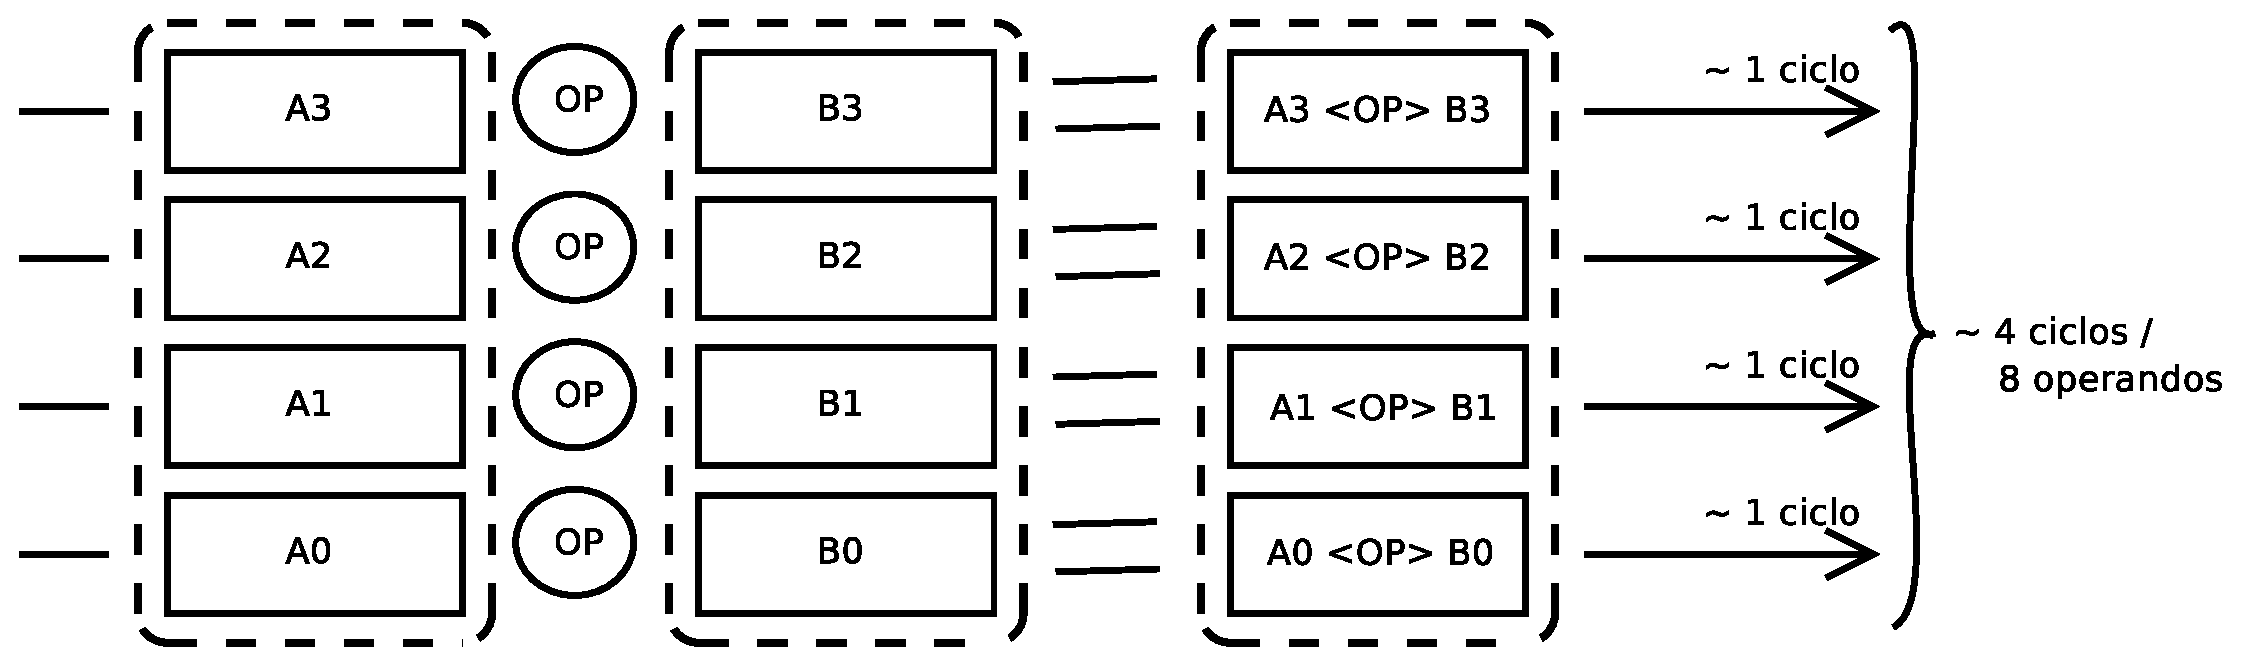
\includegraphics[width=0.85\textwidth,keepaspectratio]{sinSIMD} 
      \caption{Sin utilizar SIMD}\label{fig:sinSIMD}
    \end{figure}

    \begin{figure}[h]
      \centering
      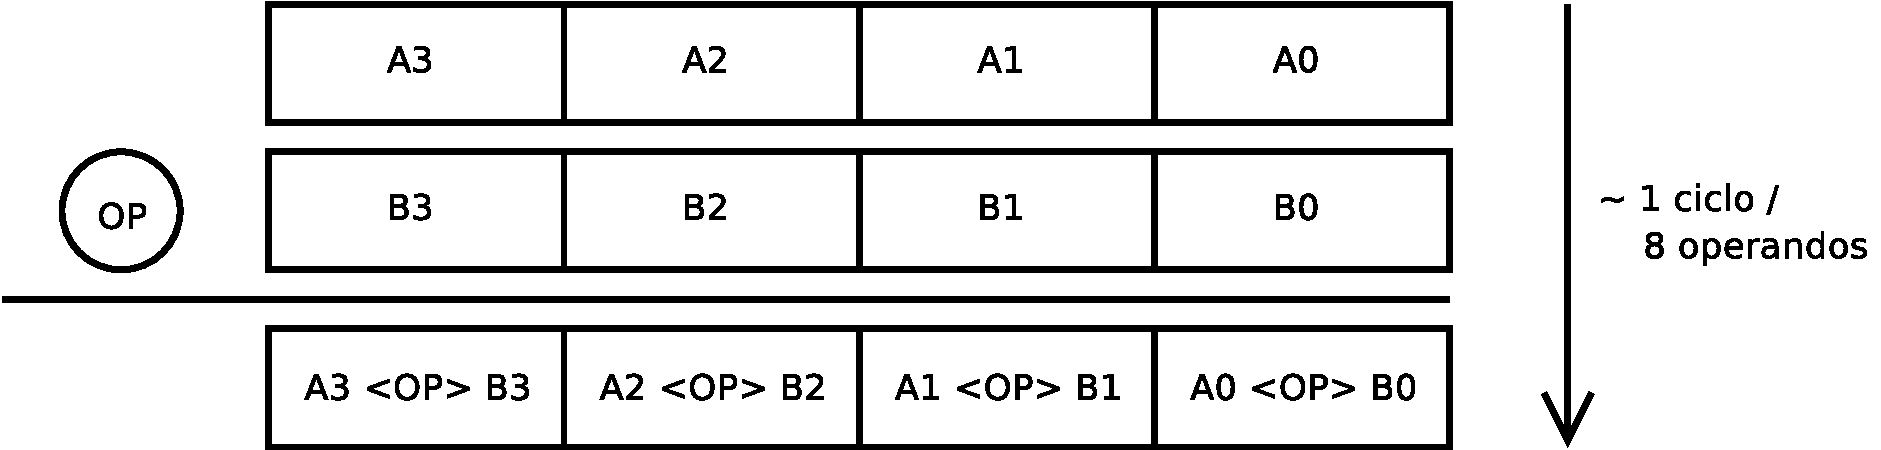
\includegraphics[width=0.85\textwidth,keepaspectratio]{conSIMD} 
      \caption{Utilizando SIMD}\label{fig:conSIMD}
    \end{figure}

    Este paralelismo intr�nseco al procesador requiere el uso de instrucciones espec�ficas del mismo, y es por ello
    dif�cilmente portable a otros sistemas. Asimismo, su utilizaci�n suele requerir el trabajo en lenguaje ensamblador, 
    con todo lo que ello supone (dificultad de mantenimiento, complejidad, etc.).

   La pr�ctica ubicuidad y potencia de estos m�todos los hacen muy atractivos. Con el fin de evitar el obst�culo
   de lo poco amigable de su uso, se ha desarrollado esta �CPU SIMD�. Sus objetivos son:
   \begin{itemize}
      \item Aislar a las rutinas de la biblioteca que deseen hacer uso de instrucciones SIMD de la implementaci�n
      real particular del procesador en cuesti�n sobre el que se est� operando. Incluso si no existe implementaci�n
      alguna, la biblioteca provee una implementaci�n gen�rica que simula su comportamiento.
      \item Homogeneizar la familia de operaciones disponibles, del mismo modo que se ha hecho con la CPU escalar.
      \item Proporcionar una abstracci�n adecuada que evite lidiar con los entresijos del lenguaje ensamblador. 
   \end{itemize} 

   \bigskip 

   Los �paquetes� SIMD tendr�n siempre una longitud de $128$ bits. En base a esto, se han definido
   tres variedades diferentes de �paquetes� de datos SIMD:
   \begin{itemize}
   \item Pares de n�meros en coma flotante de $64$ bits.
   \item Cuatro n�meros en coma flotante de $32$ bits.
   \item Ocho enteros con signo de $16$ bits.
   \end{itemize}
   Los detalles de la implementaci�n y una descripci�n m�s pormenorizada se dan en la secci�n \ref{simddigit}.



  \subsection{Repositorio de funciones}\label{basico:nuevoRepdeFuncs}
Ya en LibNumth exploramos la utilizaci�n de lo que se denomin� �repositorio de funciones�
(v�ase \cite{miproyecto}\footnote{secciones 5.6 y 4.2.3}). La idea era y sigue siendo
�hacer extensible la colecci�n de funciones \emph{sin necesidad de recompilaci�n} por parte del usuario,
y adem�s de forma sencilla�. La implementaci�n de este mecanismo en dicha versi�n de la biblioteca
era un tanto b�sica: depend�a de convenciones en el nombrado, haciendo recaer sobre el usuario
programador la carga de recordar el nombre concreto del tipo de funci�n que desease obtener. Por ejemplo:

\begin{lstlisting}[captionpos=b,basicstyle=\footnotesize,frame=shadowbox,rulesepcolor=\color{black},language=C++,numbers=left,caption=Utilizando el \textbf{antiguo} repositorio de funciones, label=lst:antiguoRepFuncs]
(...)
numth::Funciones funcs;

numth::congruentGen *LCG = new numth::congruentGen();
funcs.ponerRandom(LCG);

funcs.random()->ponerSemilla(numth::Z::convertir("323658476")); 
n = funcs.genPrimos()->leerPrimoProb(600);
(...)
\end{lstlisting}
En el anterior listado \ref{lst:antiguoRepFuncs} se aprecian los siguientes puntos:

\begin{itemize}
\item Tanto para establecer una nueva implementaci�n 
para una clase de m�todo, como para obtener la implementaci�n actual, era necesario estar al tanto del
nombre de la clase de m�todo que las instancias implementaban: \texttt{congruentGen} era un tipo de generador
de n�meros pseudo-aleatorios, y por ello deb�a utilizarse el m�todo \texttt{ponerRandom} de la clase \texttt{Funciones}, 
que representaba el repositorio. 
\item Para obtener un n�mero primo, el programador deb�a recordar que el m�todo
\texttt{genPrimos} era el indicado para obtener un puntero a una instancia generadora de primos. 
\item Incluso aunque se pretend�a seguir un patr�n de nombrado, �ste resultaba deficiente.
\item El repositorio, instancia de la clase \texttt{Funciones}, pod�a instanciarse de forma arbitraria, pese a que
conceptualmente el repositorio ha de ser �nico durante toda la ejecuci�n del programa. Este escollo se salvaba
haciendo que las instancias de las funciones contenidas en �l fueran \texttt{static}. Este simple hecho choca frontalmente
con el concepto de \textit{thread-safety}, tal como se expone en la secci�n \ref{par:datosStatic}.
\end{itemize}

Esta forma de operar no s�lo resulta tediosa y 
propensa a errores, sino tambi�n \emph{poco elegante}. La idea
es siempre que la m�quina trabaje por nosotros, no al contrario. Por si esto fuera poco, la presencia de datos
est�ticos da al traste con las aspiraciones de ejecuci�n concurrente de la biblioteca mediante hilos. 

Comparese el c�digo mostrado en el listado \ref{lst:antiguoRepFuncs} con el mostrado en el siguiente listado \ref{lst:nuevoRepFuncs}:
\begin{lstlisting}[captionpos=b,basicstyle=\footnotesize,frame=shadowbox,rulesepcolor=\color{black},language=C++,numbers=left,caption=Utilizando el \textbf{nuevo} repositorio de funciones, label=lst:nuevoRepFuncs]
(...)
mpplas::MethodsFactory& funcs(MethodsFactory::getReference());
mpplas::RandomFast* rnd;
mpplas::PrimeGen* primes;

mpplas::RandomFast* newRnd = new mpplas::CongruentGen();
funcs.setFunc(newRnd);

funcs.getFunc(rnd);
rnd->setSeed(mpplas::Z("323658476"));

funcs.getFunc(primes);
n = primes->getInteger(600);
(...)
\end{lstlisting}
Ambas porciones de c�digo son sem�nticamente equivalentes. Sin embargo:
\begin{itemize}
\item El repositorio, denominado ahora \texttt{MethodsFactory}, es ahora un \texttt{Singleton} (v�ase secci�n \ref{sec:singleton}). 
\item Se trabaja con punteros a los tipos que representan el concepto \emph{abstracto} a realizar: generar primos, obtener n�meros
pseudo-aleatorios, etc. en vez de con los tipos que en �ltima instancia implementan dichos conceptos.
\item El repositorio consiste \emph{�nicamente} de dos m�todos: \texttt{getFunc} y \texttt{setFunc}. El mecanismo
de funcionamiento, denominado \textit{autowiring}, se expone en \ref{sec:autowiring}. En este contexto, ambos
m�todos inspeccionan el tipo de las instancias que les son pasadas como par�metros a la hora de asignar
o establecer las instancias pertinentes, de forma totalmente transparente para el usuario, y garantizando \emph{en tiempo
de compilaci�n} la coherencia de dichas operaciones.
\end{itemize}

    
  \subsection{Control de errores}\label{controlDeErrores}


\section{Compilando la biblioteca}\label{estructuraGeneralDeLaLiberia}

% CAPITULO IMPLEMENTACION 

\chapter{Detalles de implementaci�n}\label{chap:detallesImpl}

\begin{flushright}
  \begin{minipage}[t]{13cm}
    \begin{flushright}
      \begin{quote}
        \emph{
          Se deben absorber los colores de la vida, pero nunca deben de
          recordarse sus detalles. Los detalles son siempre vulgares.
        }
        \begin{flushright}
          \textbf{\textemdash Oscar Wilde, El retrato de Dorian Gray}
        \end{flushright}
      \end{quote}
    \end{flushright}
  \end{minipage}
\end{flushright}

\bigskip

\begin{flushright}
  \begin{minipage}[t]{13cm}
    \begin{flushright}
      \begin{quote}
        \emph{
          Cu�date de aquel que no se molesta en los detalles.
        }
        \begin{flushright}
          \textbf{\textemdash William Feather}
        \end{flushright}
      \end{quote}
    \end{flushright}
  \end{minipage}
\end{flushright}

\bigskip

\begin{center}{\line(1,0){325}}\end{center}

%--------------------------------------------------------%
\section{Introducci�n}
 

\section{Elementos generados din�micamente}
 
  - system info
    - cpu info
    - compilation config
  - preprocesador en python
  - el cliente en python
  - el mecanismo de perfilado basado en aop


\section{Asegurando la coherencia algebraica}
- comprobaciones estataticas de caracter algebraico de parametros de templates
en la particularizaci�n de estructuras genericas


\section{El nuevo repositorio de funciones}

\section{Una nueva cpu}
- cpu vectorial


\section{La utilidad de fingir}
- mock openmp


\section{El mundo de los $64$ bits}

\section{El maestro compilador}
- scons

\section{Implementaci�n de tipos}
  \subsection{El tipo \emph{\texttt{MPPDataType}}\index{tipos!MPPDataType} }

  \subsection{Categorizaci�n algebraica}
  En la figura \ref{fig:categoriasAlgebraicas} se muestra la jerarqu�a de clases que
  modelan las categor�as algebraicas consideradas, junto con sus m�todos (est�ticos) asociados.  
  \begin{figure}[h]
    \centering
    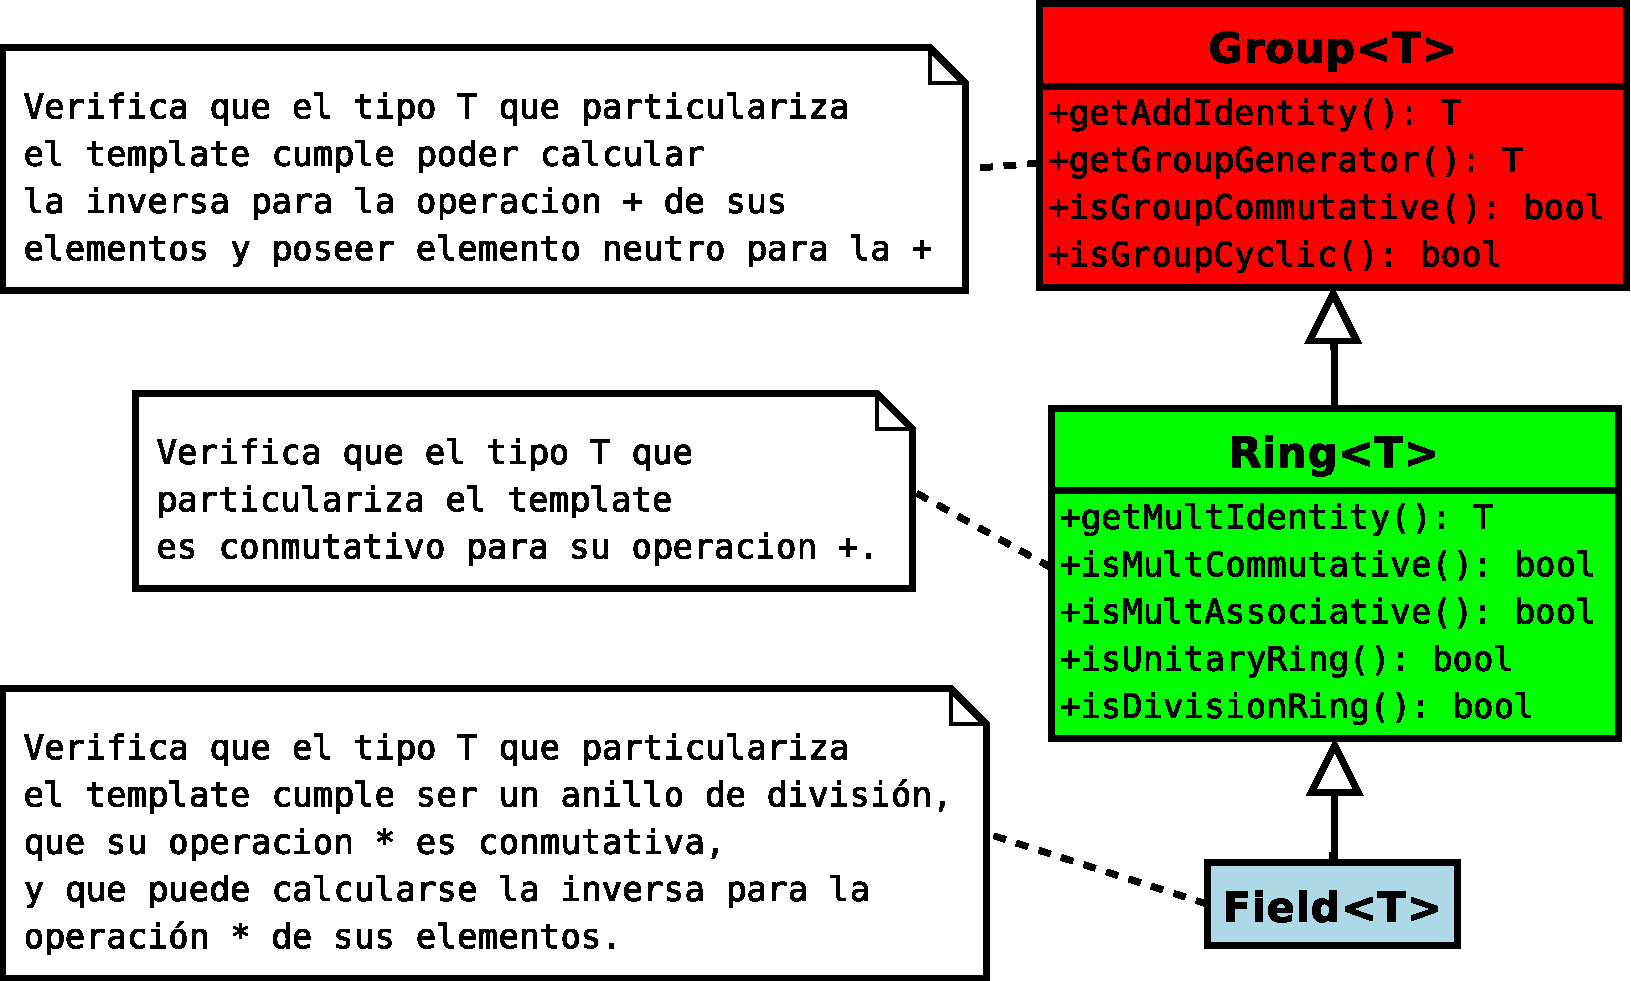
\includegraphics[width=0.95\textwidth,keepaspectratio]{categoriasAlgebraicas} 
    \caption{Categorias algebraicas}\label{fig:categoriasAlgebraicas}
  \end{figure}
  Cuando un tipo de dato de la librar�a (es decir, un hijo de \texttt{MPPDataType}) se
  encasilla dentro de esta jerarqu�a, sobre dicho tipo (representado mediante el par�metro 
  de plantilla \texttt{T}) se realizan una serie de comprobaciones, dise�adas para verificar
  que efectivamente dicho tipo cumple las condiciones impuestas por la categor�a 
  algebraica a la que aspira pertenecer. Esta serie de comprobaciones se realizan por medio
  de \emph{asertos}.



\begin{lstlisting}[captionpos=b,basicstyle=\footnotesize,frame=shadowbox,rulesepcolor=\color{black},language=C++,numbers=left,caption=STATIC\_ASSERT, label=lst:staticassert]
~Group() {
  STATIC_ASSERT( ValidateRequirements() );
}
(...)
static bool ValidateRequirements() {
  T (T::*getAddInverse)() const __attribute__ ((__unused__))  = &(T::getAddInverse) ;
  const T& (*getAddIdentity)() __attribute__ ((__unused__))  = &(T::getAddIdentity) ;
  const T& (*getGroupGenerator)() __attribute__ ((__unused__)) = &(T::getGroupGenerator) ;

  return true;
}
\end{lstlisting}


  \begin{figure}[h]
    \centering
    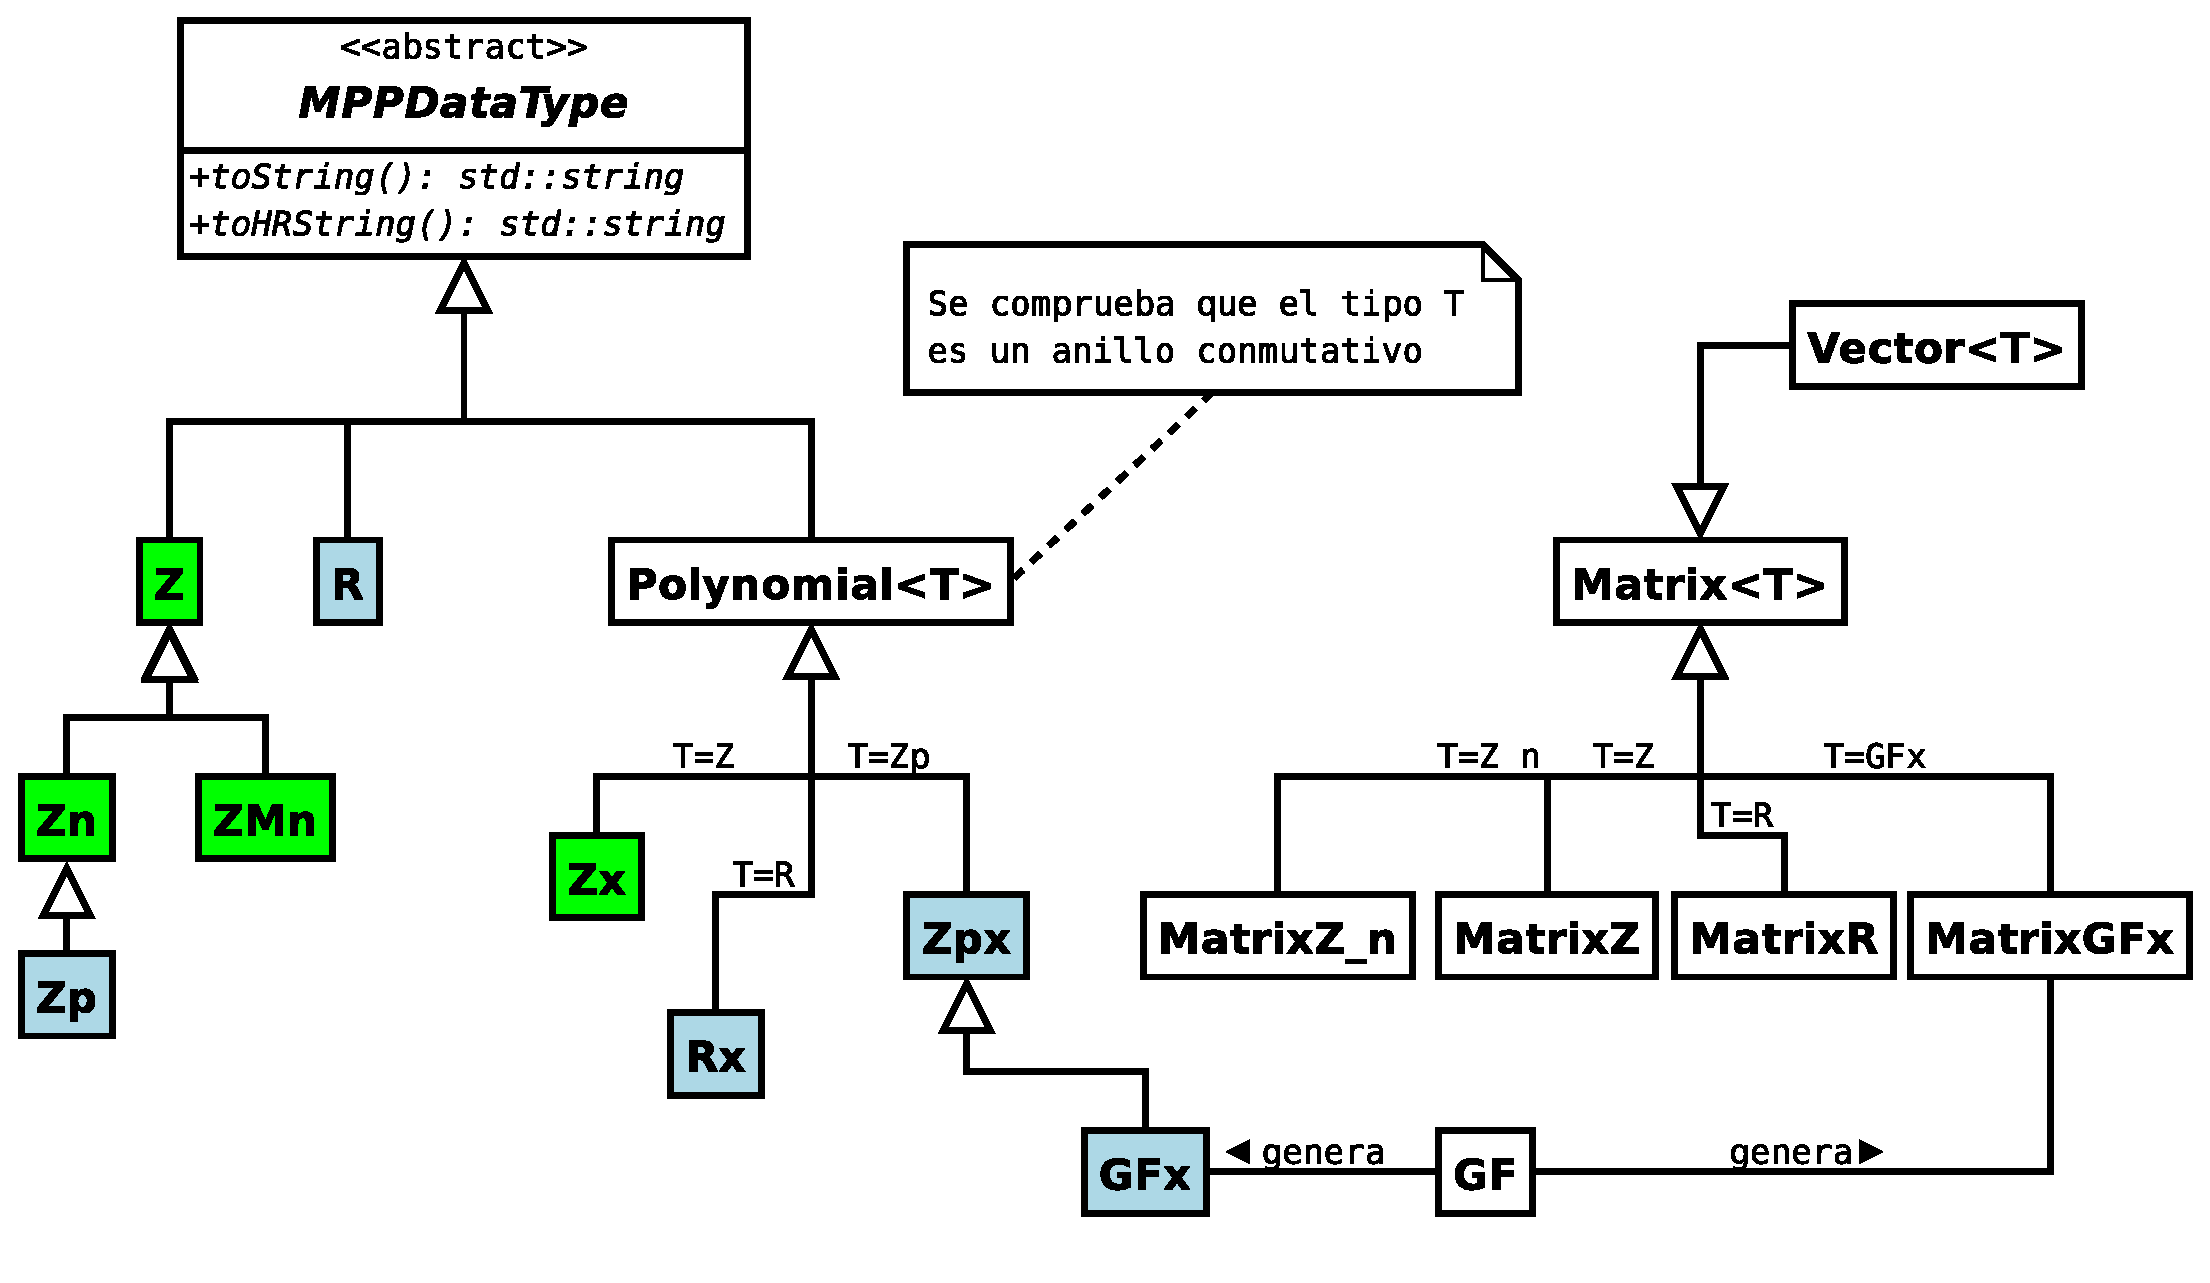
\includegraphics[width=0.95\textwidth,keepaspectratio]{categorizacionAlgebraica} 
    \caption{Categorizaci�n algebraica}\label{fig:categorizacionAlgebraica}
  \end{figure}




  \subsection{Enteros $\mathbb{Z}M_n$}\label{implZM_n}

  \subsection{Polinomios}\index{implementaci�n!polinomios}\label{impl:polinomios}
    totalmente genericos
  \subsubsection{Verificando el car�cter de $S$}
    tiene que ser como ser como minimo anillo conmutativo con unidad. Verificaciones estaticas
  \subsubsection{Operaciones dependientes de $S$}
    p ej, div en udf o  no, idem pa gcd  


  \subsection{Matrices}\index{tipos!Matrices}

% CAPITULO SOBRE FUNCIONES TRASCENDENTES

\chapter{Funciones trascendentes}\label{cap:primos}

\begin{flushright}
  \begin{minipage}[t]{13cm}
    \begin{flushright}
      \begin{quote}
        \emph{
         cita
        }
        \begin{flushright}
          \textbf{\textemdash D. Zagier}
        \end{flushright}
      \end{quote}
    \end{flushright}
  \end{minipage}
\end{flushright}

\bigskip

\begin{flushright}
  \begin{minipage}[t]{13cm}
    \begin{flushright}
      \begin{quote}
        \emph{
        cita 2
        }
        \begin{flushright}
          \textbf{\textemdash H. Montgomery}
        \end{flushright}
      \end{quote}
    \end{flushright}
  \end{minipage}
\end{flushright}

\bigskip

\begin{center}{\line(1,0){325}}\end{center}

%--------------------------------------------------------%

\section{Introducci�n}
\section{La funci�n exponencial}
  
  \subsection{Exponencial inversa: la funci�n logaritmo}
    \begin{observacion}\label{obsLog}
      Si $x \in \mathbb{R}$, existe un $n \in \mathbb{N}$ tal que
      $2^{n-1} < x \leq 2^n$. Entonces, si $y = x/2^n$, se verifica
      que $0 < y \leq 1$
    \end{observacion}

    En base a la observaci�n \ref{obsLog}, el c�lculo de $x \in
    \mathbb{R}$ se reducir�a a (utilizando los s�mbolos de dicha
    observaci�n):
    \[
      \log{(x)} = \log{(y \times 2^n)} = \log{(y)} + n \cdot \log{(2)}
    \]
    Las ventajas que de esta forma de calcula el logaritmo se
    desprenden son claras: por una parte, el c�lculo de $\log(2)$ (tambi�n denominada
    ``La constante logar�tmica'', v�ase \cite{log2}) es un problema
    ampliamente tratado y existen m�todos de gran eficiencia para su c�lculo. 
    M�s adelante se tratar� este punto en m�s profundidad.
    Por otra parte, al cumplirse $0 < y \leq 1$, el c�lculo de
    $\log{(y)}$ puede realizarse satisfactoriamente y con relativa
    efectividad utilizando la expansi�n de MacLaurin
    para la funci�n logaritmo.

    \subsubsection{La constante logar�tmica}

    


  
\section{Funciones trigonom�tricas}

  \subsection{El c�lculo de las inversas}



% CAPITULO SOBRE LAS DEMOSTRACIONES Y COMPARACI�N

\chapter{Ejemplos y comparativa}

\begin{flushright}
  \begin{minipage}[t]{13cm}
    \begin{flushright}
      \begin{quote}
        \emph{
        Las palabras son enanos, los ejemplos son gigantes.
        }
        \begin{flushright}
          \textbf{\textemdash Proverbio suizo.}
        \end{flushright}
      \end{quote}
    \end{flushright}
  \end{minipage}
\end{flushright}

\begin{center}{\line(1,0){325}}\end{center}

%--------------------------------------------------------%

 
  

% CAPITULO SOBRE LAS POSIBLES MEJORAS, AMPLIACIONES Y CRITICA

\chapter{Cr�tica}

\begin{flushright}
  \begin{minipage}[t]{13cm}
    \begin{flushright}
      \begin{quote}
        \emph{
          Become addicted to constant and never-ending self improvement.
        }
        \begin{flushright}
          \textbf{\textemdash Anthony J. D'Angelo, The College Blue Book}
        \end{flushright}
      \end{quote}
    \end{flushright}
  \end{minipage}
\end{flushright}

\begin{center}{\line(1,0){325}}\end{center}

%--------------------------------------------------------%

\section{Posibles mejoras}
  \subsection{Mayor aprovechamiento de instrucciones SIMD}
    En las operaciones con matrices.

\section{Ampliaciones}
  \subsection{Sobre Polinomios}
    \subsubsection{Factorizaci�n}
      Al igual que para la factorizaci�n de enteros, no se conoce
      un m�todo que permita realizar esta operaci�n en un tiempo razonable. Como es habitual
      en este contexto, �razonable� suele traducirse como �computable en tiempo polinomial�.
      %TODO
  \subsection{Sobre cuerpos finitos}
    En la implementaci�n actual los cuerpos finitos $\GF{p^n}$, 
    se modela $p$ como un entero de tipo \texttt{mpplas::Z}; es decir,
    un entero de precisi�n arbitraria. En la mayor�a de los casos, la caracter�stica de la precisi�n arbitraria
    no es explotada, y de hecho influye negativamente en el rendimiento. De hecho, es usual el uso de cuerpos
    finitos de la forma $\GF{2^n}$. En este caso, es posible explotar el car�cter binario de los elementos.
    Por ejemplo, la suma se reduce a una operaci�n o-exclusivo a nivel de bits. 

    En cualquier caso, la presente biblioteca se centra entorno a tipos de precisi�n arbitraria, raz�n por la cual
    esta caracter�stica tendr�a m�s cabida en otro tipo de biblioteca.


\section{Conclusiones}
  


%% PRUEBAS BORRADOR

\chapter{Pruebas, \textbf{BORRADOR}}
\section{Casos de prueba por funci�n}
\begin{itemize}
  \item divMP(vector, vector)
    \begin{itemize}
      \item[-] Ejemplo: Un entero igual a
        $79228162514264337593543950336 = 2^{32+64}$ y otro igual a 
        $4294967296 = 2^{32}$. Su divisi�n provoca a fecha 21 de Enero 
        que falle la divisi�n debido a que el tama�o del dividendo 
        disminuye m�s r�pido que de uno en uno, mientras que la guarda
        del bucle ``principal'' disminuye de uno en uno.\\
        \textbf{Soluci�n}: La guarda del bucle debe actualizarse en
        funci�n de la variaci�n de tama�o del dividendo.
    \end{itemize}
\end{itemize}

        
        

%%%%%%%%%%%%%%%%%%%%%%%%%%%%%%%%%%%%%%%%%%%%%%%%%%%%%

\bibliographystyle{proyecto}
\bibliography{bibliografia}

\printindex 

\end{document}
